
\documentclass[letterpaper,hide notes,xcolor={table,svgnames},pdftex,10pt]{beamer}
\def\showexamples{t}


%\usepackage[svgnames]{xcolor}

%% Demo talk
%\documentclass[letterpaper,notes=show]{beamer}

\usecolortheme{crane}
\setbeamertemplate{navigation symbols}{}

\usetheme{MyPittsburgh}
%\usetheme{Frankfurt}

%\usepackage{tipa}

\usepackage{hyperref}
\usepackage{graphicx,xspace}
\usepackage[normalem]{ulem}
\usepackage{multicol}
\usepackage{amsmath,amssymb,amsthm,graphicx,xspace}
\newcommand\SF[1]{$\bigstar$\footnote{SF: #1}}

\usepackage[default]{sourcesanspro}
\usepackage[T1]{fontenc}
\usepackage[scaled]{beramono}
\usepackage{tikzpagenodes}

\newcounter{tmpnumSlide}
\newcounter{tmpnumNote}


% old question code
%\newcommand\question[1]{{$\bigstar$ \small \onlySlide{2}{#1}}}
% \newcommand\nquestion[1]{\ifdefined \presentationonly \textcircled{?} \fi \note{\par{\Large \textbf{?}} #1}}
% \newcommand\nanswer[1]{\note{\par{\Large \textbf{A}} #1}}


 \newcommand\mnote[1]{%
   \addtocounter{tmpnumSlide}{1}
   \ifdefined\showcues {~\tiny\fbox{\arabic{tmpnumSlide}}}\fi
   \note{\setlength{\parskip}{1ex}\addtocounter{tmpnumNote}{1}\textbf{\Large \arabic{tmpnumNote}:} {#1\par}}}

\newcommand\mmnote[1]{\note{\setlength{\parskip}{1ex}#1\par}}

%\newcommand\mnote[2][]{\ifdefined\handoutwithnotes {~\tiny\fbox{#1}}\fi
% \note{\setlength{\parskip}{1ex}\textbf{\Large #1:} #2\par}}

%\newcommand\mnote[2][]{{\tiny\fbox{#1}} \note{\setlength{\parskip}{1ex}\textbf{\Large #1:} #2\par}}

\newcommand\mquestion[2]{{~\color{red}\fbox{?}}\note{\setlength{\parskip}{1ex}\par{\Large \textbf{?}} #1} \note{\setlength{\parskip}{1ex}\par{\Large \textbf{A}} #2\par}\ifdefined \presentationonly \pause \fi}

\newcommand\blackboard[1]{%
\ifdefined   \showblackboard
  {#1}
  \else {\begin{center} \fbox{\colorbox{blue!30}{%
         \begin{minipage}{.95\linewidth}%
           \hspace{\stretch{1}} Some space intentionally left blank; done at the blackboard.%
         \end{minipage}}}\end{center}}%
         \fi%
}



%\newcommand\q{\tikz \node[thick,color=black,shape=circle]{?};}
%\newcommand\q{\ifdefined \presentationonly \textcircled{?} \fi}

\usepackage{listings}
\lstset{basicstyle=\footnotesize\ttfamily,
	breaklines=true,
	aboveskip=15pt,
  	belowskip=15pt,
	frame=lines,
	numbers=left, basicstyle=\scriptsize, numberstyle=\tiny, stepnumber=0, numbersep=2pt
}

\usepackage{siunitx}
\newcommand\sius[1]{\num[group-separator = {,}]{#1}\si{\micro\second}}
\newcommand\sims[1]{\num[group-separator = {,}]{#1}\si{\milli\second}}
\newcommand\sins[1]{\num[group-separator = {,}]{#1}\si{\nano\second}}
\sisetup{group-separator = {,}, group-digits = true}

%% -------------------- tikz --------------------
\usepackage{tikz}
\usetikzlibrary{positioning}
\usetikzlibrary{arrows,backgrounds,automata,decorations.shapes,decorations.pathmorphing,decorations.markings,decorations.text,decorations.pathreplacing}

\tikzstyle{place}=[circle,draw=blue!50,fill=blue!20,thick, inner sep=0pt,minimum size=6mm]
\tikzstyle{transition}=[rectangle,draw=black!50,fill=black!20,thick, inner sep=0pt,minimum size=4mm]

\tikzstyle{block}=[rectangle,draw=black, thick, inner sep=5pt]
\tikzstyle{bullet}=[circle,draw=black, fill=black, thin, inner sep=2pt]

\tikzstyle{pre}=[<-,shorten <=1pt,>=stealth',semithick]
\tikzstyle{post}=[->,shorten >=1pt,>=stealth',semithick]
\tikzstyle{bi}=[<->,shorten >=1pt,shorten <=1pt, >=stealth',semithick]

\tikzstyle{mut}=[-,>=stealth',semithick]

\tikzstyle{treereset}=[dashed,->, shorten >=1pt,>=stealth',thin]

\usepackage{ifmtarg}
\usepackage{xifthen}
\makeatletter
% new counter to now which frame it is within the sequence
\newcounter{multiframecounter}
% initialize buffer for previously used frame title
\gdef\lastframetitle{\textit{undefined}}
% new environment for a multi-frame
\newenvironment{multiframe}[1][]{%
\ifthenelse{\isempty{#1}}{%
% if no frame title was set via optional parameter,
% only increase sequence counter by 1
\addtocounter{multiframecounter}{1}%
}{%
% new frame title has been provided, thus
% reset sequence counter to 1 and buffer frame title for later use
\setcounter{multiframecounter}{1}%
\gdef\lastframetitle{#1}%
}%
% start conventional frame environment and
% automatically set frame title followed by sequence counter
\begin{frame}%
\frametitle{\lastframetitle~{\normalfont(\arabic{multiframecounter})}}%
}{%
\end{frame}%
}
\makeatother

\makeatletter
\newdimen\tu@tmpa%
\newdimen\ydiffl%
\newdimen\xdiffl%
\newcommand\ydiff[2]{%
    \coordinate (tmpnamea) at (#1);%
    \coordinate (tmpnameb) at (#2);%
    \pgfextracty{\tu@tmpa}{\pgfpointanchor{tmpnamea}{center}}%
    \pgfextracty{\ydiffl}{\pgfpointanchor{tmpnameb}{center}}%
    \advance\ydiffl by -\tu@tmpa%
}
\newcommand\xdiff[2]{%
    \coordinate (tmpnamea) at (#1);%
    \coordinate (tmpnameb) at (#2);%
    \pgfextractx{\tu@tmpa}{\pgfpointanchor{tmpnamea}{center}}%
    \pgfextractx{\xdiffl}{\pgfpointanchor{tmpnameb}{center}}%
    \advance\xdiffl by -\tu@tmpa%
}
\makeatother
\newcommand{\copyrightbox}[3][r]{%
\begin{tikzpicture}%
\node[inner sep=0pt,minimum size=2em](ciimage){#2};
\usefont{OT1}{phv}{n}{n}\fontsize{4}{4}\selectfont
\ydiff{ciimage.south}{ciimage.north}
\xdiff{ciimage.west}{ciimage.east}
\ifthenelse{\equal{#1}{r}}{%
\node[inner sep=0pt,right=1ex of ciimage.south east,anchor=north west,rotate=90]%
{\raggedleft\color{black!50}\parbox{\the\ydiffl}{\raggedright{}#3}};%
}{%
\ifthenelse{\equal{#1}{l}}{%
\node[inner sep=0pt,right=1ex of ciimage.south west,anchor=south west,rotate=90]%
{\raggedleft\color{black!50}\parbox{\the\ydiffl}{\raggedright{}#3}};%
}{%
\node[inner sep=0pt,below=1ex of ciimage.south west,anchor=north west]%
{\raggedleft\color{black!50}\parbox{\the\xdiffl}{\raggedright{}#3}};%
}
}
\end{tikzpicture}
}


%% --------------------

%\usepackage[excludeor]{everyhook}
%\PushPreHook{par}{\setbox0=\lastbox\llap{MUH}}\box0}

%\vspace*{\stretch{1}

%\setbox0=\lastbox \llap{\textbullet\enskip}\box0}

\setlength{\parskip}{\fill}

\newcommand\noskips{\setlength{\parskip}{1ex}}
\newcommand\doskips{\setlength{\parskip}{\fill}}

\newcommand\xx{\par\vspace*{\stretch{1}}\par}
\newcommand\xxs{\par\vspace*{2ex}\par}
\newcommand\tuple[1]{\langle #1 \rangle}
\newcommand\code[1]{{\sf \footnotesize #1}}
\newcommand\ex[1]{\uline{Example:} \ifdefined \presentationonly \pause \fi
  \ifdefined\showexamples#1\xspace\else{\uline{\hspace*{2cm}}}\fi}

\newcommand\ceil[1]{\lceil #1 \rceil}


\AtBeginSection[]
{
   \begin{frame}
       \frametitle{Outline}
       \tableofcontents[currentsection]
   \end{frame}
}



\pgfdeclarelayer{edgelayer}
\pgfdeclarelayer{nodelayer}
\pgfsetlayers{edgelayer,nodelayer,main}

\tikzstyle{none}=[inner sep=0pt]
\tikzstyle{rn}=[circle,fill=Red,draw=Black,line width=0.8 pt]
\tikzstyle{gn}=[circle,fill=Lime,draw=Black,line width=0.8 pt]
\tikzstyle{yn}=[circle,fill=Yellow,draw=Black,line width=0.8 pt]
\tikzstyle{empty}=[circle,fill=White,draw=Black]
\tikzstyle{bw} = [rectangle, draw, fill=blue!20, 
    text width=4em, text centered, rounded corners, minimum height=2em]
    
    \newcommand{\CcNote}[1]{% longname
	This work is licensed under the \textit{Creative Commons #1 3.0 License}.%
}
\newcommand{\CcImageBy}[1]{%
	\includegraphics[scale=#1]{creative_commons/cc_by_30.pdf}%
}
\newcommand{\CcImageSa}[1]{%
	\includegraphics[scale=#1]{creative_commons/cc_sa_30.pdf}%
}
\newcommand{\CcImageNc}[1]{%
	\includegraphics[scale=#1]{creative_commons/cc_nc_30.pdf}%
}
\newcommand{\CcGroupBySa}[2]{% zoom, gap
	\CcImageBy{#1}\hspace*{#2}\CcImageNc{#1}\hspace*{#2}\CcImageSa{#1}%
}
\newcommand{\CcLongnameByNcSa}{Attribution-NonCommercial-ShareAlike}

\newenvironment{changemargin}[1]{% 
  \begin{list}{}{% 
    \setlength{\topsep}{0pt}% 
    \setlength{\leftmargin}{#1}% 
    \setlength{\rightmargin}{1em}
    \setlength{\listparindent}{\parindent}% 
    \setlength{\itemindent}{\parindent}% 
    \setlength{\parsep}{\parskip}% 
  }% 
  \item[]}{\end{list}} 




\title{Lecture 5 --- Concurrency and Parallelism }

\author{Jeff Zarnett \& Patrick Lam \\ \small \texttt{jzarnett@uwaterloo.ca} \texttt{patrick.lam@uwaterloo.ca}}
\institute{Department of Electrical and Computer Engineering \\
  University of Waterloo}
\date{\today}

\begin{document}

\begin{frame}
  \titlepage

 \end{frame}

\part{Limits}
\begin{frame}
\partpage
\begin{center}
	
\includegraphics[width=0.6\textwidth]{images/limit.jpg}\\
	``Push it to the limit!''\\
	( \url{https://www.youtube.com/watch?v=kZu5iDTtNg0})
\end{center}
\end{frame}

\begin{frame}
\frametitle{Writing Scalable Code}

Think about the worst case run-time performance of the algorithm. 

An algorithm that's $O(n^{3})$ scales so much worse than one that's $O(n)$... 

Trying to do an insertion sort on a small array is fine (actually... recommended); doing it on a huge array is madness.

Choosing a good algorithm is very important if we want it to scale. 

\end{frame}

\begin{frame}
\frametitle{Big-O Complexity}
\begin{center}
	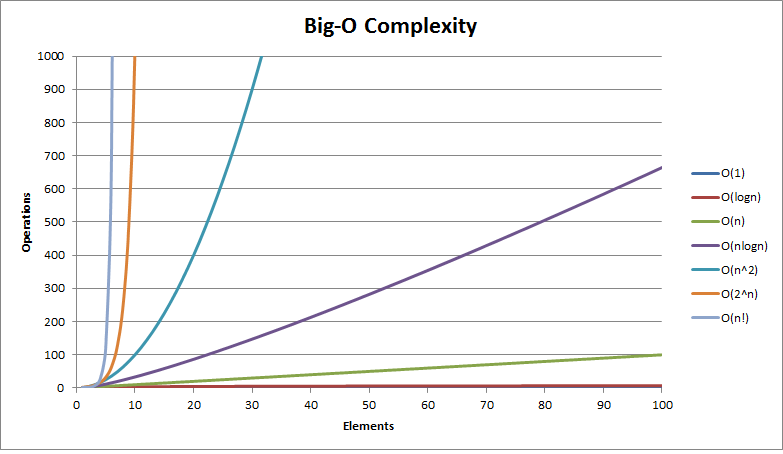
\includegraphics[width=0.75\textwidth]{images/big-o-complexity}
\end{center}

\end{frame}
\begin{frame}
  \frametitle{Parallelism versus Concurrency}

  Before we talk about parallelism, let's distinguish it from concurrency.

  {\bf Parallelism}

  Two or more tasks are \structure{parallel}\\ \hspace*{2em} if they are running at the same time. 

  Main goal: run tasks as fast as possible. 

  Main concern: \structure{dependencies}.
  \vfill
  {\bf Concurrency}

  Two or more tasks are \structure{concurrent}\\ \hspace*{2em} if the ordering of the two tasks is not 
  predetermined. 

  Main concern: \structure{synchronization}.

\end{frame}

\begin{frame}
  \frametitle{Limitations of Speedups}

    Our main focus is parallelization.\\[1em]
  \begin{itemize}
    \item Most programs have a sequential part and a parallel part; and,\\[1em]
    \item Amdahl's Law answers, ``what are the limits to parallelization?''
  \end{itemize}

\end{frame}



\begin{frame}
\frametitle{Visualizing Amdahl's Law}

  \hspace*{2em}\begin{minipage}{.8\textwidth}
  $S$: fraction of serial runtime in a serial execution.

  $P$: fraction of parallel runtime in a serial execution.

  Therefore, $S + P = 1$.\\[2em]

  With 4 processors, best case, what can happen to the following runtime?
  \end{minipage}

  \hspace*{5em}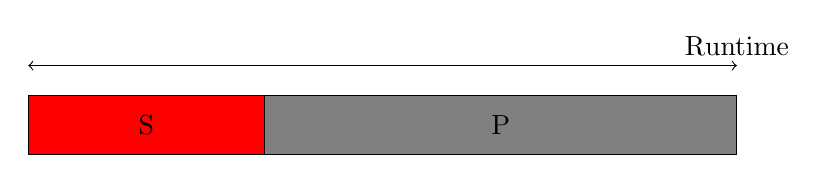
\begin{tikzpicture}
   \draw[<->] (-1.5,0.75) -- (7.5,0.75) node[above] {Runtime};
   \draw (0,0) node[rectangle, fill=red, minimum height=0.75cm, minimum width=3cm,draw] {S};
   \draw (4.5,0) node[rectangle, fill=gray, minimum height=0.75cm, minimum width=6cm,draw] {P};
  \end{tikzpicture}
\end{frame}

\begin{frame}
  \frametitle{Visualizing Amdahl's Law}

  \hspace*{5em}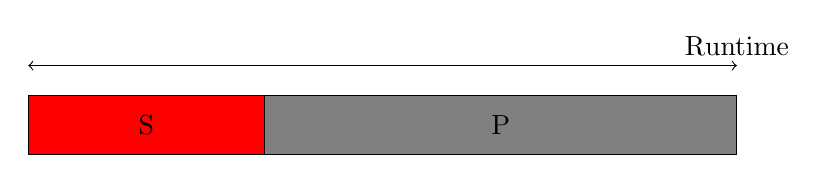
\begin{tikzpicture}
   \draw[<->] (-1.5,0.75) -- (7.5,0.75) node[above] {Runtime};
   \draw (0,0) node[rectangle, fill=red, minimum height=0.75cm, minimum width=3cm,draw] {S};
   \draw (4.5,0) node[rectangle, fill=gray, minimum height=0.75cm, minimum width=6cm,draw] {P};
  \end{tikzpicture}
  \vfill
  We want to split up the parallel part over 4 processors
  \vfill
  \hspace*{5em}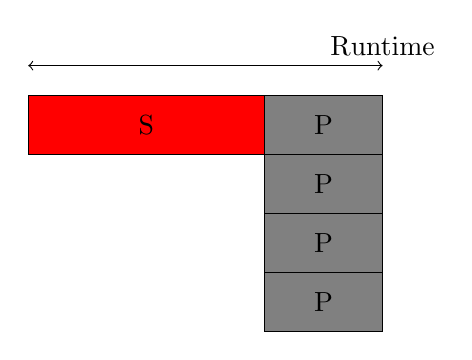
\begin{tikzpicture}
   \draw[<->] (-1.5,0.75) -- (3,0.75) node[above] {Runtime};
   \draw (0,0) node[rectangle, fill=red, minimum height=0.75cm, minimum width=3cm,draw] {S};
   \draw (2.25,0) node[rectangle, fill=gray, minimum height=0.75cm, minimum width=1.5cm,draw] {P};
   \draw (2.25,-0.75) node[rectangle, fill=gray, minimum height=0.75cm, minimum width=1.5cm,draw] {P};
   \draw (2.25,-1.5) node[rectangle, fill=gray, minimum height=0.75cm, minimum width=1.5cm,draw] {P};
   \draw (2.25,-2.25) node[rectangle, fill=gray, minimum height=0.75cm, minimum width=1.5cm,draw] {P};
  \end{tikzpicture}
\end{frame}

\begin{frame}
  \frametitle{Obey the Law}

\Large
$T_s$: time for the program to run in serial

$N$: number of processors/parallel executions

$T_p$: time for the program to run in parallel
\vfill
  \begin{itemize}
    \item Under perfect conditions, get $N$ speedup for $P$
  \end{itemize}
\vfill

  \begin{center}
$T_p = T_s \cdot (S + \frac{P}{N})$
  \end{center}
\end{frame}

\begin{frame}
  \frametitle{Obey the Law}

  \hspace*{3em} How much faster can we make the program?

  \begin{eqnarray*}
  \mbox{\em speedup} &=& \frac{T_s}{T_p}\\
                     &=& \frac{T_s}{T_S \cdot (S + \frac{P}{N})}\\
                     &=& \frac{1}{S + \frac{P}{N}}
  \end{eqnarray*}
  \vfill
  \hspace*{3em} (assuming no overhead for parallelizing; or costs near
  zero)

\end{frame}

\begin{frame}
  \frametitle{Fixed-Size Problem Scaling, \\ Varying Fraction of Parallel Code}

  \begin{center}
    \hspace*{2em}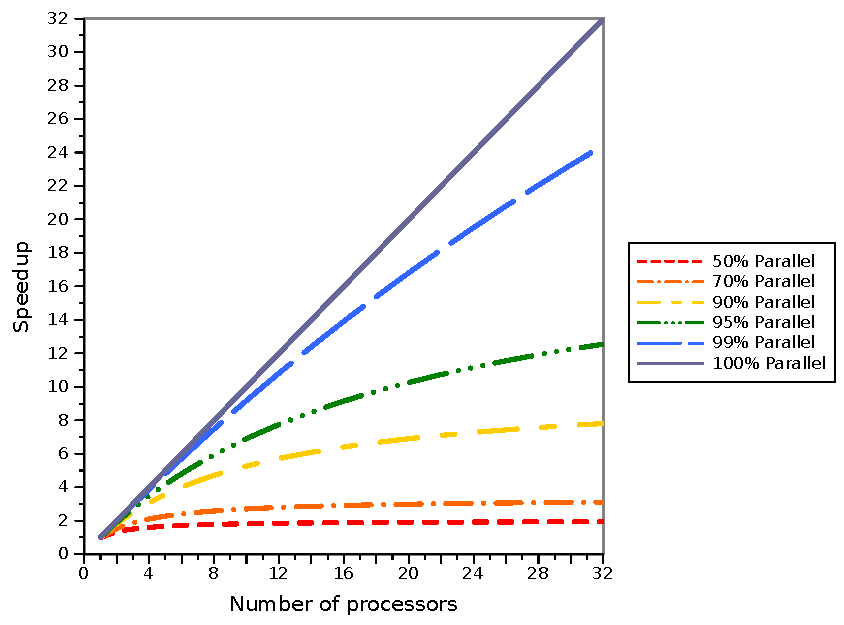
\includegraphics[scale=0.68]{images/parallel-scaling.pdf}
  \end{center}
\end{frame}


\begin{frame}
  \frametitle{Amdahl's Law}

 \hspace*{2em}Replace $S$ with $(1 - P)$:

  \begin{center}
    \structure{$\mbox{\em speedup} = \frac{1}{(1 - P) + \frac{P}{N}}$}
  \end{center}
  \vfill
  \begin{center}
    $\mbox{\em maximum speedup} = \frac{1}{(1 - P)}$, since $\frac{P}{N} \rightarrow 0$
  \end{center}

As you might imagine, the asymptotes in the previous graph are bounded by the
  maximum speedup.
\end{frame}

\begin{frame}
\frametitle{Speedup Example}


Suppose: a task that can be executed in 5~s, containing a parallelizable loop.

Initialization and recombination code in this routine requires 400~ms. 

So with one processor executing, it would take about 4.6~s to execute the loop. 

Split it up and execute on two processors: about 2.3~s to execute the loop. 

Add to that the setup and cleanup time of 0.4~s and we get a total time of 2.7~s. 

Completing the task in 2.7~s rather than 5~s represents a speedup of about~46\%.

\end{frame}


\begin{frame}
\frametitle{Amdahl's Law on the 5~s Task}

Applying this formula to the example:

\begin{center}
	\begin{tabular}{l|l}
	\textbf{Processors} & \textbf{Run Time (s)} \\ \hline
	1 & 5\\
	2 & 2.7\\
	4 & 1.55\\
	8 & 0.975\\
	16 & 0.6875 \\
	32 & 0.54375 \\
	64 & 0.471875 \\
	128 & 0.4359375\\
	\end{tabular}
\end{center}

\end{frame}

 
\begin{frame}
\frametitle{Observations on the 5~s Task}

1. Diminishing returns as we add more processors.

2. Converges on 0.4~s.

The most we could speed up this code is by a factor of $\frac{5}{0.4}\approx 12.5$.

But that would require infinite processors (and therefore infinite money).

\end{frame}

\begin{frame}
  \frametitle{Assumptions behind Amdahl's Law}

    We assume:
    \begin{itemize}
    \item problem size is fixed (we'll see this soon);
    \item program/algorithm behaves the same on 1 processor and on $N$ processors;
    \item that we can accurately measure runtimes---\\ ~~i.e. that overheads don't matter.
    \end{itemize}
  
\end{frame}

\begin{frame}
  \frametitle{Amdahl's Law Generalization}

  \hspace*{2em} The program may have many parts, each of which we can tune to
  a different degree.\\[1em]

  Let's generalize Amdahl's Law.\\[1em]

  $f_1, f_2, \ldots, f_n$: fraction of time in part $n$

  $S_{f_1}, S_{f_n}, \ldots, S_{f_n}$: speedup for part $n$

  \vfill
  \begin{center}
  \structure{\[\mbox{\em speedup} = \frac{1}{\frac{f_1}{S_{f_1}} + \frac{f_2}{S_{f_2}} + \ldots +
    \frac{f_n}{S_{f_n}}}\]}
  \end{center}
\end{frame}


\begin{frame}
  \frametitle{Application (1)}

  \hspace*{2em} 
Consider a program with 4 parts in the following scenario:\\[2em]
    \begin{tabular}{r|r|r|r}
    \multicolumn{2}{l}{} & \multicolumn{2}{c}{Speedup} \\
    Part & Fraction of Runtime & Option 1 & Option 2\\
    \hline
    1 & 0.55 & 1  & 2\\
    2 & 0.25 & 5  & 1\\
    3 & 0.15 & 3  & 1\\
    4 & 0.05  & 10 & 1\\
  \end{tabular}

~\\[2em]
  We can implement either Option 1 or Option 2. \\
  Which option is better?

\end{frame}

\begin{frame}
  \frametitle{Application (2)}


  \hspace*{2em} ``Plug and chug'' the numbers:\\[1em]

  {\bf Option 1} \vspace*{-2em}

  \[ \mbox{\em speedup} = \frac{1}{0.55 + \frac{0.25}{5} + \frac{0.15}{3} + \frac{0.05}{5}}
    = 1.53  \]
~\\[1em]
  {\bf Option 2} \vspace*{-2em}

   \[\mbox{\em speedup} = \frac{1}{\frac{0.55}{2} + 0.45} = 1.38 \hspace*{5.5em}\]


\end{frame}

\begin{frame}
  \frametitle{Empirically estimating parallel speedup P}

  \hspace*{2em} Useful to know, don't have to commit to memory:
  \vfill
  \[P_{\mbox{\scriptsize estimated}} = \frac{\frac{1}{\mbox{\em speedup}}-1}{\frac{1}{N}-1}\]
  \vfill
  \hspace*{2em} \begin{minipage}{.8\textwidth} \begin{itemize}
    \item Quick way to guess the fraction of parallel code
    \item Use $P_{\mbox{\scriptsize estimated}}$ to predict speedup for a different number of processors
  \end{itemize} \end{minipage}
\end{frame}

\begin{frame}
  \frametitle{Summary of Amdahl's Law}

\hspace*{2em} Important to focus on the part of the program with most impact.\\[1em]

\hspace*{2em} Amdahl's Law:\\[1em]
\hspace*{2em}
  \begin{itemize}
    \item estimates perfect performance gains from
          parallelization (under assumptions); but,
    \vfill
    \item only applies to solving a \structure{fixed problem size} in the
          shortest possible period of time
  \end{itemize}
\end{frame}

\begin{frame}
  \frametitle{Gustafson's Law: Formulation}

\hspace*{2em} 
\begin{tabbing}
  $n$:~~~~~~ \= problem size\\[.1em]

  $S(n)$: \> fraction of serial runtime for a parallel execution\\[.1em]

  $P(n)$: \> fraction of parallel runtime for a parallel execution\\
\end{tabbing}


\begin{eqnarray*}
T_p &=& S(n) + P(n) = 1 \\
T_s &=& S(n) + N \cdot P(n) 
\end{eqnarray*}

\[ \mbox{\em speedup} = \frac{T_s}{T_p} \]
\end{frame}

\begin{frame}
  \frametitle{Gustafson's Law}

\hspace*{2em}
  \structure{$speedup = S(n) + N \cdot P(n)$}\\[1em]

  Assuming the fraction of runtime in serial part decreases as $n$ increases,
  the speedup approaches $N$.


Yes! Large problems can be efficiently parallelized. (Ask Google.)

\end{frame}

\begin{frame}
  \frametitle{Driving Metaphor}

  {\bf Amdahl's Law}
  
  Suppose you're travelling between 2 cities 90~km apart. If you travel for an
  hour at a constant speed less than 90 km/h, your average will never equal
  90~km/h, even if you energize after that hour.
  \vfill
  {\bf Gustafson's Law}

  Suppose you've been travelling at a constant speed less than 90~km/h. Given
  enough distance, you can bring your average up to 90~km/h.
\end{frame}

\part{Parallelization Techniques}
\begin{frame}
\partpage
\end{frame}

\begin{frame}
\frametitle{Lock It Down}
The more locks and locking we need, the less scalable the code is going to be. 

You may think of the lock as a resource. 
The more threads or processes that are looking to acquire that lock, the more ``resource contention'' we have.

And thus more waiting and coordination are going to be necessary.

\end{frame}

\begin{frame}
\frametitle{``We have a new enemy...''}

Assuming we're not working with an embedded system where all memory is statically allocated in advance, there will be dynamic memory allocation. 

The memory allocator is often centralized and may support only one thread allocating or deallocating at a time (using locks to ensure this). 

This means it does not necessarily scale very well.

There are some techniques for dynamic memory allocation that allow these things to work in parallel.


\end{frame}


\begin{frame}
\frametitle{Doing Lines}

Multiprocessor (multicore) processors have some hardware that tries to keep the data consistent between different pipelines and caches.

 More processors, more threads means more work is necessary to keep these things in order.

\end{frame}



\begin{frame}
\frametitle{Everybody Into the Pool}

If we have a pool of workers, the application just submits units of work, and then on the other side these units of work are allocated to workers. 

The number of workers will scale based on the available hardware. 

This is neat as a programming practice: as the application developer we don't care quite so much about the underlying hardware. 

Let the operating system decide how many workers there should be, to figure out the optimal way to process the units of work.

\end{frame}


\part{Parallelization Technique: Threads vs Processes}
\begin{frame}
\partpage
\end{frame}


\begin{frame}[fragile]
  \frametitle{Background}


  Recall the difference between \structure{processes} and 
          \structure{threads}:
  \begin{itemize}
    \item Threads are basically light-weight processes which piggy-back on
          processes' address space.
  \end{itemize} ~\\
  Traditionally (pre-Linux 2.6) you had to use {\tt fork}~(for~processes) and {\tt clone} (for threads).


\end{frame}

\begin{frame}[fragile]
  \frametitle{History}


    Developers mostly used {\tt fork} before there was a standardized way to create threads ({\tt clone} was non-standards-complient).

  For performance reasons, along with ease and consistency, we'll use
  \structure{Pthreads}.

  {\tt fork} creates a new process.
      \begin{itemize}
        \item Drawbacks?
        \item Benefits?
      \end{itemize}
  
\end{frame}

\begin{frame}[fragile]
  \frametitle{Benefit: {\tt fork} is Safer and More Secure Than Threads}

  \begin{enumerate}
    \item Each process has its own virtual address space:
      \begin{itemize}
        \item Memory pages are not copied, they are copy-on-write---
        \item Therefore, uses less memory than you would expect.
      \end{itemize}
    \item Buffer overruns or other security holes do not expose other~processes.
    \item If a process crashes, the others can continue.
  \end{enumerate}~\\[1em]
  {\bf Example:} In the Chrome browser, each tab is a separate process.
\end{frame}

\begin{frame}[fragile]
  \frametitle{Drawback of Processes: Threads are Easier and Faster}

  \begin{itemize}
    \item Interprocess communication (IPC) is more complicated and slower than interthread
          communication.
      \begin{itemize}
        \item Need to use operating system utilities (pipes, semaphores, shared
              memory, etc) instead of thread library (or just memory reads and writes).
      \end{itemize}
    \item Processes have much higher startup, shutdown and synchronization cost.
    \item And, \structure{Pthreads}/\structure{C++11 threads} fix issues\\ with {\tt clone} and provide a
          uniform interface for most systems {\bf (Assignment 1)}.
  \end{itemize}

\end{frame}

\begin{frame}[fragile]
  \frametitle{Appropriate Time to Use Processes}


  If your application is like this:
  \begin{itemize}
    \item Mostly independent tasks, with little or no communication.
    \item Task startup and shutdown costs are negligible compared to overall runtime.
    \item Want to be safer against bugs and security holes.
  \end{itemize}
  Then processes are the way to go. \\[1em]


\end{frame}


\begin{frame}
\frametitle{Thread Motivation}
Why threads instead of a new process?

Primary motivation is: performance.

\begin{enumerate}
	\item Creation: 10$\times$ faster.
	\item Terminating and cleaning up a thread is faster.
	\item Switch time: 20\% of process switch time.
	\item Shared memory space (no need for IPC).
	\item Lets the UI be responsive.
\end{enumerate}

\end{frame}

\begin{frame}
\frametitle{Common Usage of Threads}

\begin{enumerate}
	\item \textbf{Foreground and Background Work}
	\item \textbf{Asynchronous processing}
	\item \textbf{Speed of Execution}
	\item \textbf{Modular Structure}
\end{enumerate}

\end{frame}

\begin{frame}
\frametitle{Thread Drawbacks}

There is no protection between threads in the same process. 

One thread can easily mess with the memory being used by another. 

This once again brings us to the subject of co-ordination, which will follow the discussion of threads.

Also, if any thread encounters an error, the whole process might be terminated by the operating system.

\end{frame}

\begin{frame}[fragile]
  \frametitle{Results: Threads Offer a Speedup of 6.5 over {\tt fork}}


  Here's a benchmark between {\tt fork} and Pthreads on a laptop, creating and
  destroying 50,000 threads:
  \vfill
  \begin{lstlisting}[basicstyle=\scriptsize]
jon@riker examples master % time ./create_fork 
0.18s user 4.14s system 34% cpu 12.484 total
jon@riker examples master % time ./create_pthread 
0.73s user 1.29s system 107% cpu 1.887 total
  \end{lstlisting}
  \vfill
  Clearly Pthreads incur much lower overhead than {\tt fork}.
  
\end{frame}


\begin{frame}
\frametitle{More Detail: Processes and Threads}
A \alert{process} is an
instance of a computer program that contains program code and its own
address space, stack, registers, and resources (file handles, etc).  

A
\alert{thread} usually belongs to a process. 

The most important point
is that it shares an address space with its parent process, hence
variables and code as well as resources.


\end{frame}



\begin{frame}
\frametitle{Threads}

Each thread has its own:
\begin{enumerate}
	\item Thread execution state.
	\item Saved thread context when not running.
	\item Execution stack.
	\item Local variables.
	\item Access to the memory and resources of the process.
\end{enumerate}


\end{frame}



\begin{frame}
\frametitle{Threads and Processes}

\begin{center}
	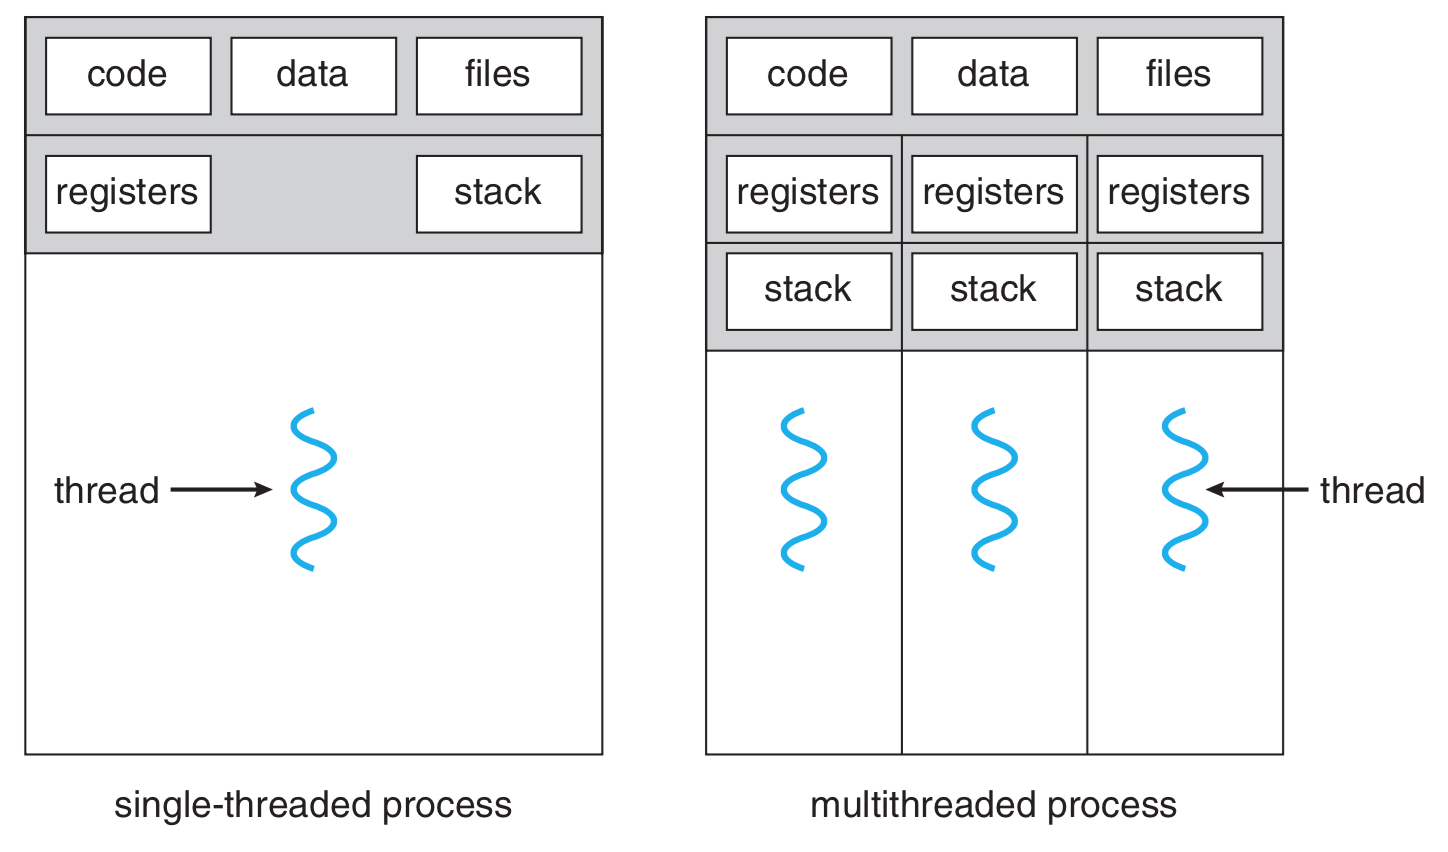
\includegraphics[width=0.625\textwidth]{images/mthread2.png}
\end{center}

All the threads of a process share the state and resources of the process. If one thread opens a file, other threads in that process can also access that file.

My usual example: file transfer program...

\end{frame}

\begin{frame}
  \frametitle{Thread implementations: Software and Hardware Threads}


  {\bf Software Thread:}

  What you program with (e.g. with {\tt pthread\_create()} or {\tt std::thread()}). \vfill

  Corresponds to a stream of instructions executed by the processor. \vfill

  On a single-core, single-processor machine, someone has to multiplex the CPU to
  execute multiple threads concurrently; only one thread runs at a time.

  \vfill
  {\bf Hardware Thread:}

  Corresponds to virtual (or real) CPUs in a system. Also known as strands. \vfill

  Operating system must multiplex software threads onto hardware threads, but 
  can execute more than one software thread at once.


\end{frame}

\begin{frame}
  \frametitle{Thread Model---1:1 (Kernel-level Threading)}


    Simplest possible threading implementation.
    \vfill
    The kernel schedules threads on different processors;
      \begin{itemize}
        \item NB: Kernel involvement required to take advantage of a multicore system.
      \end{itemize}
    \vfill
    Context switching involves system call overhead.
    \vfill
    Used by Win32, POSIX threads for Windows and Linux.
    \vfill
    Allows concurrency and parallelism.

\end{frame}

\begin{frame}
  \frametitle{Thread Model---N:1 (User-level Threading)}

    All application threads map to a single kernel thread.
    \vfill
    Quick context switches, no need for system call.
    \vfill
    Cannot use multiple processors, only for concurrency.
      \begin{itemize}
        \item Why would you use user threads?
      \end{itemize}
    \vfill
    Used by GNU Portable Threads.
\end{frame}

\begin{frame}
  \frametitle{Thread Model---M:N (Hybrid Threading)}

    Map $M$ application threads to $N$ kernel threads.
    \vfill
    A compromise between the previous two models.
    \vfill
    Allows quick context switches and the use of multiple processors.
    \vfill
    Requires increased complexity:
    \begin{itemize}
        \item Both library and kernel must schedule.
        \item Schedulers may not coordinate well together.
        \item Increases likelihood of priority inversion\\ \hspace*{2em} (recall from Operating Systems).
      \end{itemize}
    \vfill
    Used by Windows 7 threads.
\end{frame}

\begin{frame}[fragile]
  \frametitle{Example System---Physical View}
  
  \begin{center}
  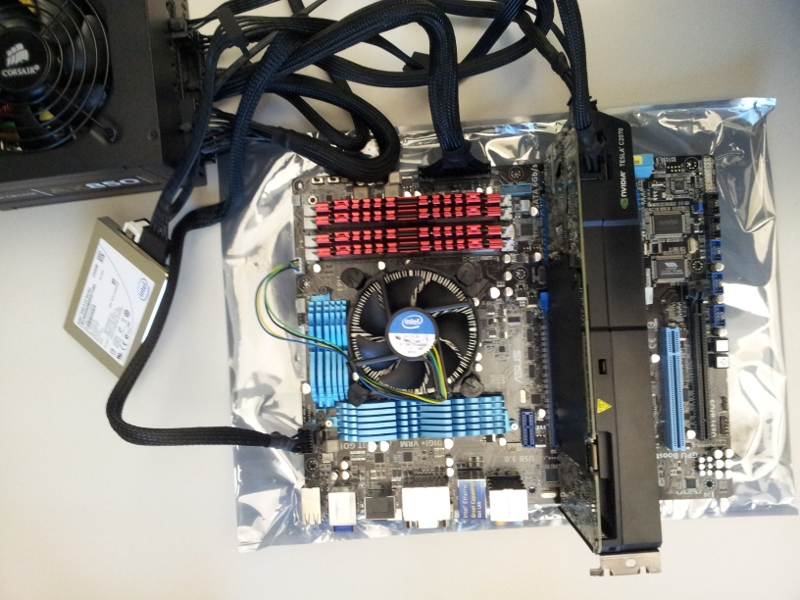
\includegraphics[scale=0.25]{images/computer-parts}
  \end{center}

  \begin{itemize}
    \item Only one physical CPU
  \end{itemize}
\end{frame}

\begin{frame}[fragile]
  \frametitle{Example System---System View}

  \scriptsize
  \begin{lstlisting}
jon@ece459-1 ~ % egrep 'processor|model name' /proc/cpuinfo 
processor : 0
model name: Intel(R) Core(TM) i7-2600K CPU @ 3.40GHz
processor : 1
model name: Intel(R) Core(TM) i7-2600K CPU @ 3.40GHz
processor : 2
model name: Intel(R) Core(TM) i7-2600K CPU @ 3.40GHz
processor : 3
model name: Intel(R) Core(TM) i7-2600K CPU @ 3.40GHz
processor : 4
model name: Intel(R) Core(TM) i7-2600K CPU @ 3.40GHz
processor : 5
model name: Intel(R) Core(TM) i7-2600K CPU @ 3.40GHz
processor : 6
model name: Intel(R) Core(TM) i7-2600K CPU @ 3.40GHz
processor : 7
model name: Intel(R) Core(TM) i7-2600K CPU @ 3.40GHz
  \end{lstlisting}

  \begin{itemize}
    \item Many processors
  \end{itemize}
\end{frame}



\end{document}

